\documentclass[conference]{IEEEtran}
\IEEEoverridecommandlockouts
% The preceding line is only needed to identify funding in the first footnote. If that is unneeded, please comment it out.
% \usepackage{cite}
% Enables Portuguese Brasil
%\usepackage[portuguese]{babel}
%encoding
% Enables code listing
\usepackage{listings}
%--------------------------------------
\usepackage[T1]{fontenc}
\usepackage[utf8]{inputenc}
%--------------------------------------
%Enables the use of greek letter without a math context
\usepackage{textgreek}
%--------------------------------------
%Enables hiperlinks
\usepackage[hidelinks]{hyperref}
%--------------------------------------

\usepackage{amsmath,amssymb,amsfonts}
\usepackage{algorithmic}
\usepackage{graphicx}
\usepackage{textcomp}
\usepackage{xcolor}

% The code style
\usepackage{color}
\definecolor{codegreen}{rgb}{0,0.6,0}
\definecolor{codegray}{rgb}{0.5,0.5,0.5}
\definecolor{codepurple}{rgb}{0.58,0,0.82}
\definecolor{backcolour}{rgb}{0.95,0.95,0.92}

\lstdefinestyle{mystyle}{
	backgroundcolor=\color{backcolour},   
	commentstyle=\color{codegreen},
	keywordstyle=\color{magenta},
	numberstyle=\tiny\color{codegray},
	stringstyle=\color{codepurple},
	basicstyle=\footnotesize,
	breakatwhitespace=false,         
	breaklines=true,                 
	captionpos=b,                    
	keepspaces=true,                 
	numbers=left,                    
	numbersep=2pt,                  
	showspaces=false,                
	showstringspaces=false,
	showtabs=false,                  
	tabsize=2
}
\lstset{style=mystyle}
%---------------------------------------


\def\BibTeX{{\rm B\kern-.05em{\sc i\kern-.025em b}\kern-.08em
    T\kern-.1667em\lower.7ex\hbox{E}\kern-.125emX}}
\begin{document}
\title{Ontologies for emotions classification}
\author{André Furlan - UNESP - Universidade Estadual Paulista "Júlio de Mesquita Filho"}
\date{2019-10-27}
\maketitle

\begin{abstract}
A short explanation on how to make a java application based on ontologies and how to model this in order to get an usable knowledge base.
\end{abstract}

\begin{IEEEkeywords}
ontologies, java, application, emotions, knowledge graph, owl
\end{IEEEkeywords}

\section{Introduction}
	Sometimes it is hard to known what is the exact intentions behind the expressions of someone. There is so many faces and body details that must be observed \cite{ekman2001telling} that is almost impossible to a non-trained classify the current person intentions or feelings. This article shows how to build an ontology, export and finally integrate it with the java programming language.
	
	All the resulting sources (and more) derived from this article are available at \textbf{\url{https://github.com/ensismoebius/ontologies}}.
\section{Tools needed}
	First of all an ontology editor must be installed, of course you can edit the ontologies by hand as well but this is a hard and tedious task. \textbf{Protégé} (\url{https://protege.stanford.edu/}) are recommended because it is a free open-source ontology editor and have a plenty of plugins that hopefully will help.\\
	\textbf{Java Development Kit} is needed as well, along with a good \textbf{java IDE}, in this article \textbf{Eclipse IDE} was the chosen one, optionally \textbf{Maven} dependency manager may be installed.
\section{Building up the ontology}
Anger, contempt, fear, happiness and lying has a wide range of emotions involved \cite{ekman2001telling} \cite{ekman1974detecting} so build an ontology for that will help the system to infer the correlations.

For the sake of this article \textbf{it is important to save the ontology in RDF format}.

Begin adding to ontology the chosen characteristics like in the figure \ref{fig:maincharac} this is what we want to know.
\begin{figure}[bpht]
	\centering
	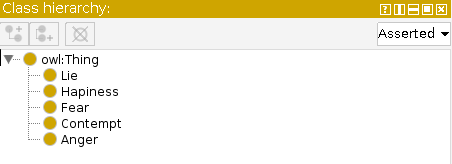
\includegraphics[width=0.7\linewidth]{mainCharac}
	\caption{Main characteristics}
	\label{fig:maincharac}
\end{figure}
The these characteristics are composed by a number of emotions sometimes diferent classifications may have some similar emotions \cite{ekman2001telling}. To tackle this difficult a new class must be created: \textbf{EmotionsSignals} (figure \ref{fig:emotinalSinals}). 
\begin{figure}[bpht]
	\centering
	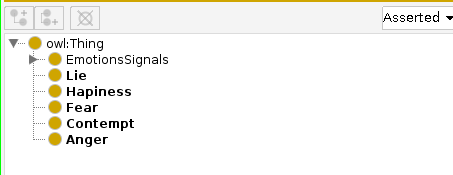
\includegraphics[width=0.7\linewidth]{emotinalSinals}
	\caption{Emotions signals}
	\label{fig:emotinalSinals}
\end{figure}

This class express a body and communicational signals some person may exhibit while talking. Subdividing \textbf{EmotionsSignals} using categories like \textbf{Hands}, \textbf{Head}, etc. The hierarchy ends like the figure \ref{fig:allEmotinalSinals} shows.
\begin{figure}[bpht]
	\centering
	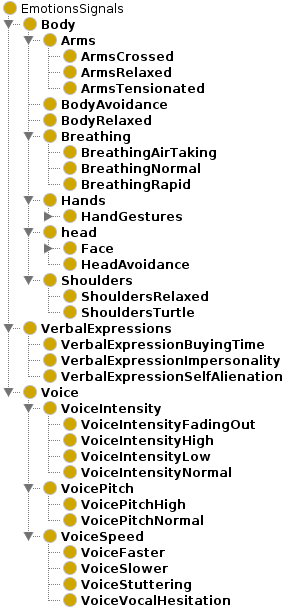
\includegraphics[width=0.5\linewidth]{allEmotinalSinals}
	\caption{Emotions signals sub classes}
	\label{fig:allEmotinalSinals}
\end{figure}
Having the defined hierarchy, the next step is to bind this main characteristics to emotions signals. It is done by creating what is called \textbf{object properties}. To do that go to "object properties" tab  inside "Entities" tab (figure \ref{fig:objectproperties}) and create \textbf{hasCaracteristic} property. The \textbf{hasCaracteristic} property was chosen arbitrary.
\begin{figure}[bpht]
	\centering
	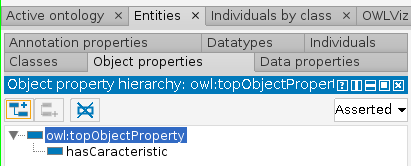
\includegraphics[width=0.7\linewidth]{objectProperties}
	\caption{Object properties tab}
	\label{fig:objectproperties}
\end{figure}
Finally, go to "classes" tab and select one by one the main characteristics (\textit{Lie} for example) and using the \textbf{SubClass} add option bind emotions signals using the \textbf{object retriction editor} like in the figure \ref{fig:emotionscharacteristics}.
\begin{figure}[bpht]
	\centering
	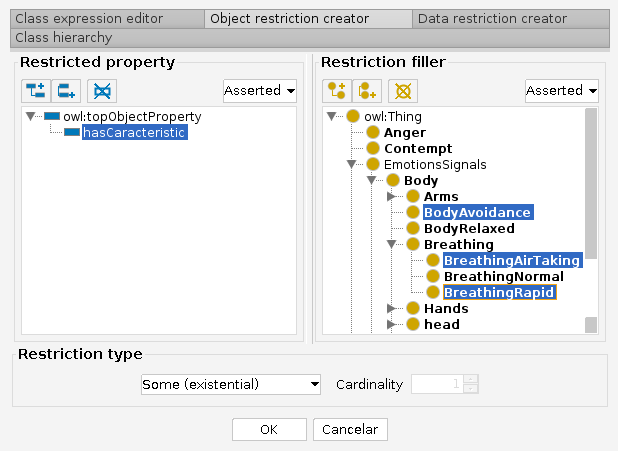
\includegraphics[width=1\linewidth]{emotionsCharacteristics}
	\caption{Binding emotions signals}
	\label{fig:emotionscharacteristics}
\end{figure}

\subsection{Building the "Lie"}
According to \cite{ekman1974detecting} and \cite{ekman2001telling} a lie may be constituted by \textbf{at least by 3} of the factors shown in the figure \ref{fig:lie}.
\begin{figure}[bpht]
	\centering
	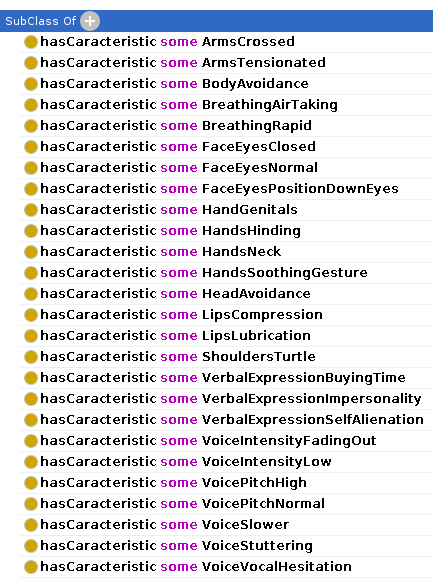
\includegraphics[width=0.7\linewidth]{lie}
	\caption{Building the Lie class}
	\label{fig:lie}
\end{figure}

\subsection{Building the "Anger"}
According to \cite{ekman2001telling} the anger may be constituted by \textbf{at least by 3} of the factors shown in the figure \ref{fig:anger}.
\begin{figure}[bpht]
	\centering
	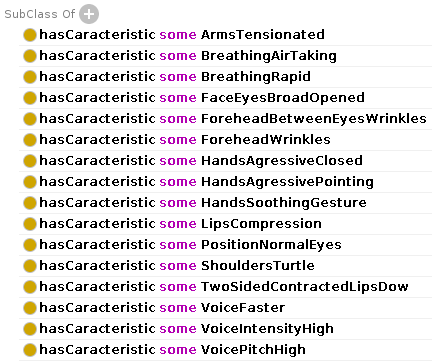
\includegraphics[width=0.7\linewidth]{anger}
	\caption{Building the Anger class}
	\label{fig:anger}
\end{figure}

\subsection{Building the "Happiness"}
According to \cite{ekman2001telling} the happiness may be constituted by \textbf{at least by 3} of the factors shown in the figure \ref{fig:happiness}.
\begin{figure}[bpht]
	\centering
	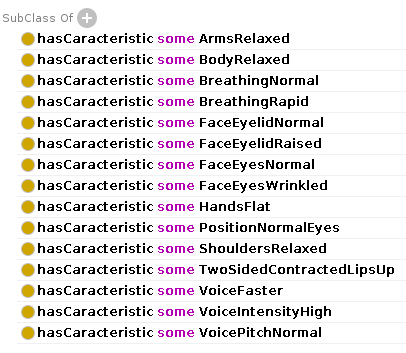
\includegraphics[width=0.7\linewidth]{happiness.png}
	\caption{Building the Happiness class}
	\label{fig:happiness}
\end{figure}

\subsection{Building the "Fear"}[bpht]
According to \cite{ekman2001telling} the fear may be constituted by \textbf{at least by 3} of the factors shown in the figure \ref{fig:fear}.
\begin{figure}[bpht]
	\centering
	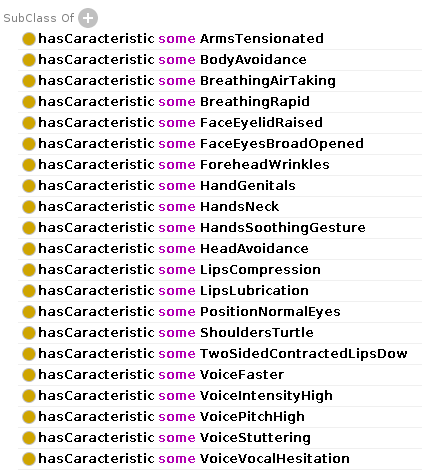
\includegraphics[width=0.7\linewidth]{fear}
	\caption{Building the Fear class}
	\label{fig:fear}
\end{figure}

\subsection{Building the "Contempt"}[bpht]
According to \cite{ekman2001telling} the contempt may be constituted by \textbf{at least by 3} of the factors shown in the figure \ref{fig:contempt}.
\begin{figure}[bpht]
	\centering
	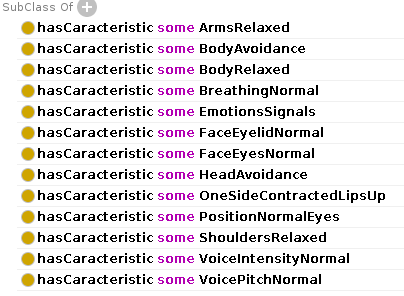
\includegraphics[width=0.7\linewidth]{contempt}
	\caption{Building the Contempt class}
	\label{fig:contempt}
\end{figure}

\textbf{Do not forget to save the ontology in RDF format.}

\section{SPARQL}
With the ontology ready a way to retrieve the main characteristics given some emotions signals is mandatory if the target is a system that can classify if a person is angry, if its lying, happy, etc.

That is where the SPARQL enters: Activating the SPARQL editor at Protégé (window $\rightarrow$ tabs $\rightarrow$ SPARQL Query) it is possible to run against the ontology some queries that are going to return the desired data.

At the current application the needed data are:
\begin{itemize}
	\item Emotions signals available using listing \ref{lst:emo}.
	\item The main characteristics given some emotions signals using listing \ref{lst:charct}.
\end{itemize}

Note that at the listing \ref{lst:charct} the \textbf{:ArmsRelaxed} and \textbf{:BodyAvoidance} statements are just examples for a query, it is possible to put more or fewer parameters as the necessity appears.
\begin{lstlisting}[language=SPARQL, caption={Getting Emotions signals available}, label={lst:emo}]
PREFIX rdf: <http://www.w3.org/1999/02/22-rdf-syntax-ns#>
PREFIX owl: <http://www.w3.org/2002/07/owl#>
PREFIX rdfs: <http://www.w3.org/2000/01/rdf-schema#>
PREFIX xsd: <http://www.w3.org/2001/XMLSchema#>
PREFIX : <http://www.semanticweb.org/ensismoebius/ontologies/2019/9/tellingLies#>

SELECT  DISTINCT ?name  WHERE { 
   ?directSub rdfs:subClassOf ?super ;
   rdfs:subClassOf [ 
        rdf:type owl:Restriction ;
             owl:onProperty :hasCaracteristic;
             owl:someValuesFrom ?name
   ] .
   FILTER( ?name != :EmotionsSignals )
}
ORDER BY (?name)
\end{lstlisting}

\begin{lstlisting}[language=SPARQL, caption={Getting the main characteristics given some emotions signals}, label={lst:charct}]
PREFIX rdf: <http://www.w3.org/1999/02/22-rdf-syntax-ns#>
PREFIX owl: <http://www.w3.org/2002/07/owl#>
PREFIX rdfs: <http://www.w3.org/2000/01/rdf-schema#>
PREFIX xsd: <http://www.w3.org/2001/XMLSchema#>
PREFIX : <http://www.semanticweb.org/ensismoebius/ontologies/2019/9/tellingLies#>

SELECT DISTINCT ?directSub 
WHERE { 
	?directSub rdfs:subClassOf ?super ;
		rdfs:subClassOf [ 
		rdf:type owl:Restriction ;
		owl:onProperty :hasCaracteristic ;
		owl:someValuesFrom :ArmsRelaxed
	] .
	?directSub rdfs:subClassOf ?super ;
		rdfs:subClassOf [ 
		rdf:type owl:Restriction ;
		owl:onProperty :hasCaracteristic ;
		owl:someValuesFrom :BodyAvoidance
	] .
}
\end{lstlisting}

\section{Programming the application}
The ontology will be read using the following libraries:
\begin{itemize}
	\item jena-arq, version 3.13.0
	\item jena-core, version 3.13.0
	\item owlapi-distribution, version 3.5.1
	\item org.semanticweb.hermit, version 1.3.8.4
\end{itemize}
It is possible to download these libraries manually but \textbf{Maven} are recommended because there is \textbf{a lot} of dependencies.

\begin{lstlisting}[language=XML, caption={Needed libraries}, label={lst:dependecies}]
<dependency>
	<groupId>net.sourceforge.owlapi</groupId>
	<artifactId>owlapi-distribution</artifactId>
	<version>3.5.1</version>
</dependency>

<dependency>
	<groupId>com.hermit-reasoner</groupId>
	<artifactId>org.semanticweb.hermit</artifactId>
	<version>1.3.8.4</version>
</dependency>

<dependency>
	<groupId>org.apache.jena</groupId>
	<artifactId>jena-core</artifactId>
	<version>3.13.0</version>
</dependency>

<dependency>
	<groupId>org.apache.jena</groupId>
	<artifactId>jena-arq</artifactId>
	<version>3.13.0</version>
</dependency>
\end{lstlisting}
After all that the programming task is trivial: Given a \textbf{set of emotions} signals return the \textbf{respective main characteristics} if any.

In this work excluding the graphical interface the important part of the programming are shown at listing \ref{lst:availableSignals} and \ref{lst:felling}.
\begin{lstlisting}[language=java, caption={Retrieve all available signals method}, label={lst:availableSignals}]
	public ArrayList<String> getSignals() throws OWLOntologyCreationException {

	String queryString = "PREFIX rdf: <http://www.w3.org/1999/02/22-rdf-syntax-ns#>\n"
	+ "PREFIX owl: <http://www.w3.org/2002/07/owl#>\n"
	+ "PREFIX rdfs: <http://www.w3.org/2000/01/rdf-schema#>\n"
	+ "PREFIX xsd: <http://www.w3.org/2001/XMLSchema#>\n"
	+ "PREFIX : <http://www.semanticweb.org/ensismoebius/ontologies/2019/9/tellingLies#>\n"
	+ "SELECT  DISTINCT ?name  WHERE { ?directSub rdfs:subClassOf ?super ;"
	+ "rdfs:subClassOf [ rdf:type owl:Restriction ;"
	+ "owl:onProperty :hasCaracteristic; owl:someValuesFrom ?name] ."
	+ "	FILTER( ?name != :EmotionsSignals )} order by (?name)";
	
	Query query = QueryFactory.create(queryString);
	QueryExecution qexec = QueryExecutionFactory.create(query, model);
	
	ArrayList<String> resultsList = new ArrayList<String>();
	ResultSet results = qexec.execSelect();
	while (results.hasNext()) {
		QuerySolution qsol = results.nextSolution();
		resultsList.add(qsol.get("name").toString());
	}
	
	qexec.close();
	
	return resultsList;
}
\end{lstlisting}

\begin{lstlisting}[language=java, caption={Retrieve characteristics}, label={lst:felling}]
	public ArrayList<String> getFelling(ArrayList<String> signals) throws OWLOntologyCreationException {
	
	String queryString = "PREFIX rdf: <http://www.w3.org/1999/02/22-rdf-syntax-ns#>\n"
	+ "PREFIX owl: <http://www.w3.org/2002/07/owl#>\n"
	+ "PREFIX rdfs: <http://www.w3.org/2000/01/rdf-schema#>\n"
	+ "PREFIX xsd: <http://www.w3.org/2001/XMLSchema#>\n"
	+ "PREFIX : <http://www.semanticweb.org/ensismoebius/ontologies/2019/9/tellingLies#>\n"
	+ "SELECT DISTINCT ?directSub " + "WHERE { ";
		
		for (String signal : signals) {
			queryString += "?directSub rdfs:subClassOf ?super ;" + "rdfs:subClassOf [" + "rdf:type owl:Restriction ;"
			+ "owl:onProperty :hasCaracteristic ;" + "owl:someValuesFrom <" + signal + ">] .";
		}
		
		queryString += "}";
	
	Query query = QueryFactory.create(queryString);
	QueryExecution qexec = QueryExecutionFactory.create(query, model);
	
	ArrayList<String> resultsList = new ArrayList<String>();
	ResultSet results = qexec.execSelect();
	while (results.hasNext()) {
		try {
			QuerySolution qsol = results.nextSolution();
			resultsList.add(qsol.get("directSub").toString());
		} catch (NullPointerException e) {
			continue;
		}
	}
	
	qexec.close();
	return resultsList;
}
\end{lstlisting}
The final application looks like the figure \ref{fig:app}.
\begin{figure}[bpht]
	\centering
	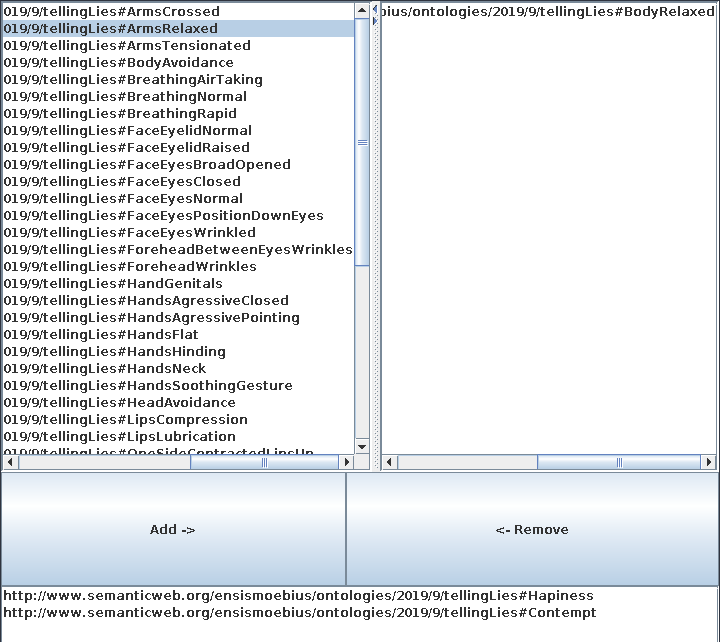
\includegraphics[width=1\linewidth]{app}
	\caption{Final application screenshot}
	\label{fig:app}
\end{figure}


\bibliography{bibliography.bib}
\bibliographystyle{alpha}

\end{document}